\documentclass[a4paper,12pt]{article}
\usepackage{HomeWorkTemplate}
\usepackage{circuitikz}
\usepackage[shortlabels]{enumitem}
\usepackage{hyperref}
\usepackage{tikz}
\usepackage{amsmath}
\usepackage{amssymb}
\usepackage{tcolorbox}
\usepackage{xepersian}
\settextfont{XB Niloofar}
\usepackage{changepage}
\newcounter{subproblemcounter}
\setcounter{subproblemcounter}{1}
\newcommand{\problem}[1]
{
	\subsection*{
		تمرین
		#1
	}
}
\newcommand{\subproblem}{
	\textbf{\harfi{subproblemcounter})}\stepcounter{subproblemcounter}
}


\begin{document}
\handout
{پردازش زبان‌های طبیعی}
{احسان‌الدین عسگری}
{نیم‌سال اول 1400\lr{-}1401}
{اطلاعیه}
{امین کشیری، فاطمه توحیدیان، سید علیرضا موسوی}
{۹۷۱۰۱۰۲۶ - ۹۷۰۰۳۵۴ - ۹۷۱۲۳۴۵۶}
{تمرین سری اول}


\section*{روند اجرای کد}

در این تمرین سعی شده است تا بتوانیم وقایع و علائم بورسی را از متن استخراج کنیم. 
منطق اصلی کد ما می‌تواند به سه قسمت اصلی تقسیم شود. در قسمت اول، به کمک کلمات کلیدی 
از پیش تعیین شده‌ای، قسمت‌هایی از متن را به دست می‌آوریم که قسمتی از یک واقعه باشند. در قسمت 
دوم، هر قسمت را بررسی می‌کنیم و سعی می‌کنیم متن کامل واقعه را به دست آوریم. در قسمت سوم نیز وقایع تکراری 
را حذف می‌کنیم و در صورتی که بتوانیم بعضی از وقایع‌ را با هم ترکیب می‌کنیم تا واقعه بهتری 
را پیدا کنیم.

دسته‌بندی اتفاقات داخل متن، به صورت زیر صورت گرفته است: 
\begin{enumerate}
    \item \textbf{نماد}
    
    نمادهای معاملاتی در بورس ایران
    \item \textbf{شرکت}
    
    نام شرکت‌های بورسی ایران 
    \item \textbf{اعلان}
    
    اصطلاحات اداری همانند گزارش، اطلاعیه و ...
	\item \textbf{تحلیل}
	
	اصطلاحات خاص بورسی و تحلیلی مانند تحلیل تکنیکال، واگرایی و ...
	\item \textbf{شخصیت}
	
	  اتفاقات مربوط به شخصیت‌های حاضر در بازار مانند نوسان‌گیر، بازیگر و
	  ...
	\item  \textbf{واقعه}
	
	سایر وقایع مهم بورسی که در دسته های بالا جای نگیرند و وقایع مختلف بورسی را نشان می‌دهند. مانند صف خرید، تقسیم سود، مجمع عمومی و ...
\end{enumerate}

دقت کنید که این دسته‌ها لزوما کل اتفاقات را افراز نمی‌کنند. برای مثال ممکن است در یک 
واقعه، یک نماد بورسی نیز وجود داشته باشد، و در این حالت ما هردوی این اتفاقات را گزارش می‌کنیم. برای برخی از وقایع 
تنها قسمتی از متن را به عنوان واقعه گزارش می‌دهیم، اما برخی وقایع پیچیده ترند و سعی می‌کنیم 
اجزای دیگری از آن را نیز خروجی دهیم. برای مثال، برای ورودی زیر، وقایع را به همراه 
فاعل آن‌ها پیدا می‌کنیم: 


\begin{center}
	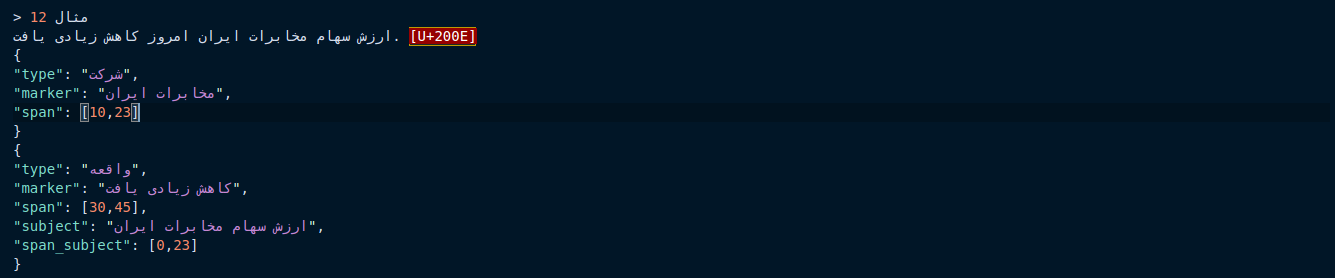
\includegraphics[scale=0.5, trim ={0 0 17cm 0}, clip]{images/12.png}
\end{center}


برای آشنایی بیشتر با خروجی کد ما، می‌توانید مثال‌های زیر را ببینید. 

\begin{center}
	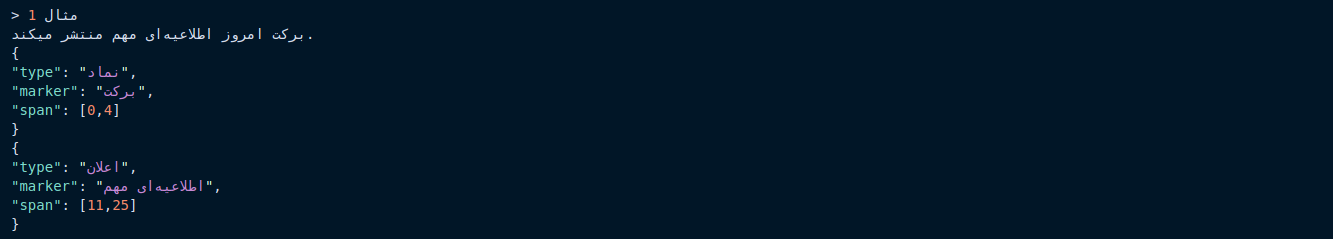
\includegraphics[scale=0.5, trim ={0 0 17cm 0}, clip]{images/1.png}

	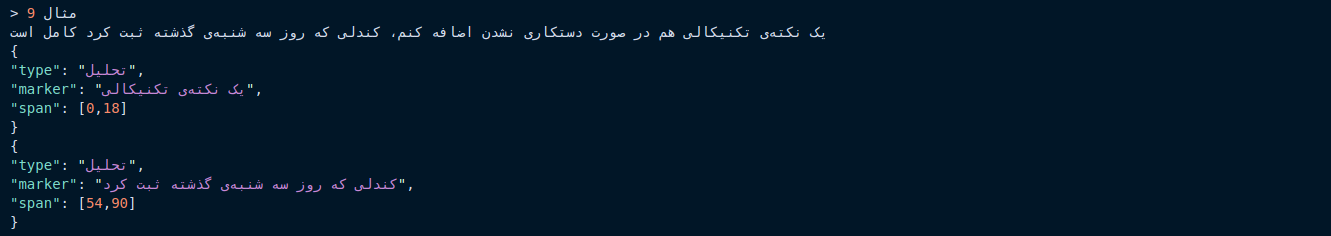
\includegraphics[scale=0.5, trim ={0 0 17cm 0}, clip]{images/9.png}

	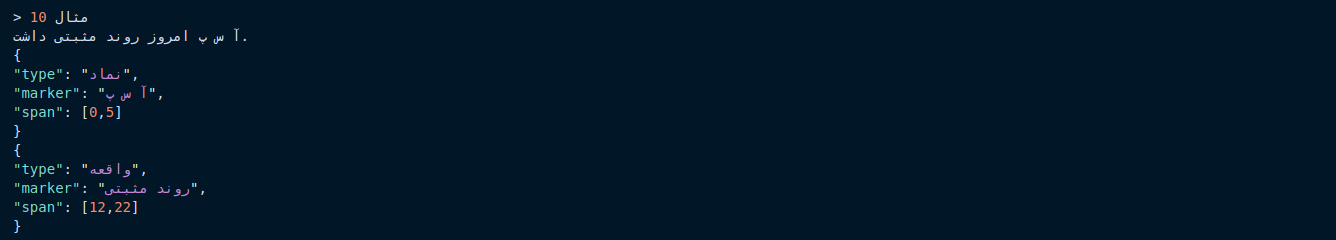
\includegraphics[scale=0.5, trim ={0 0 17cm 0}, clip]{images/10.png}

	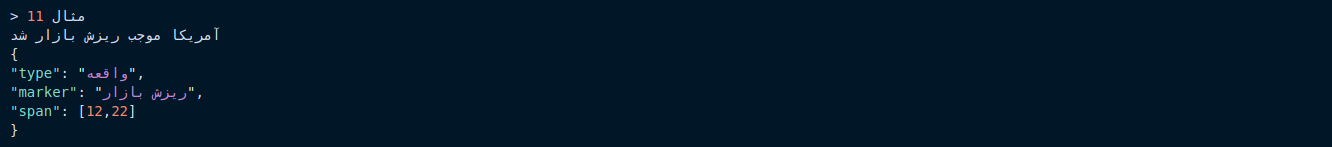
\includegraphics[scale=0.5, trim ={0 0 17cm 0}, clip]{images/11.png}

	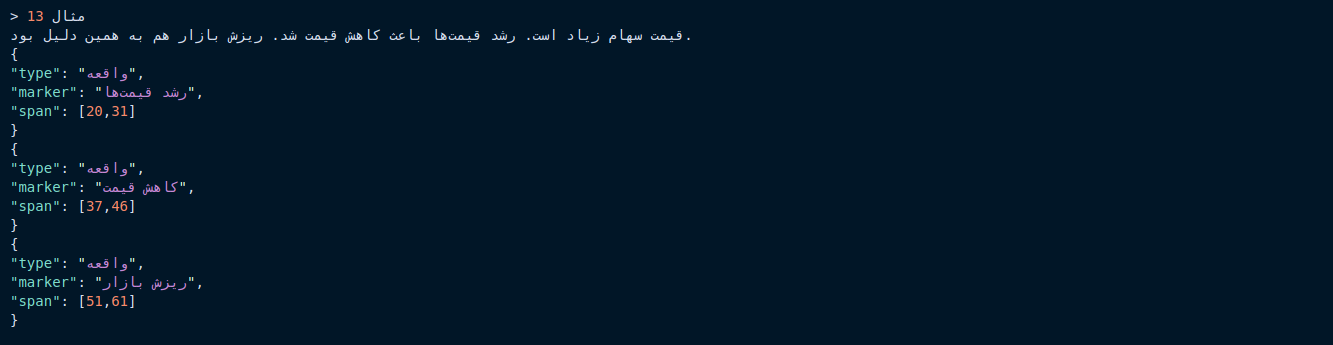
\includegraphics[scale=0.5, trim ={0 0 17cm 0}, clip]{images/13.png}

	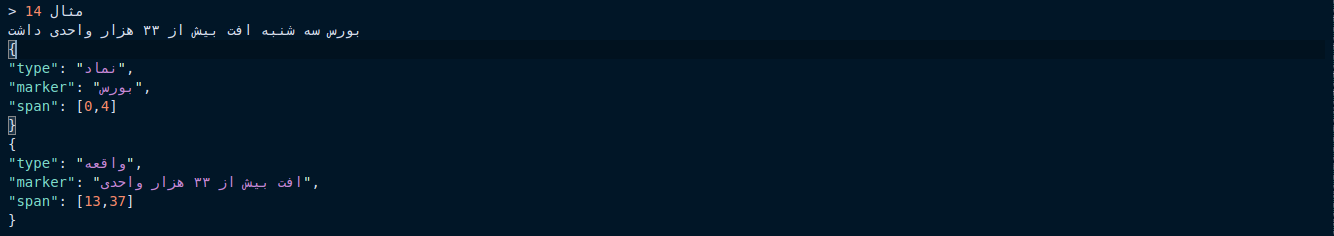
\includegraphics[scale=0.5, trim ={0 0 17cm 0}, clip]{images/14.png}

	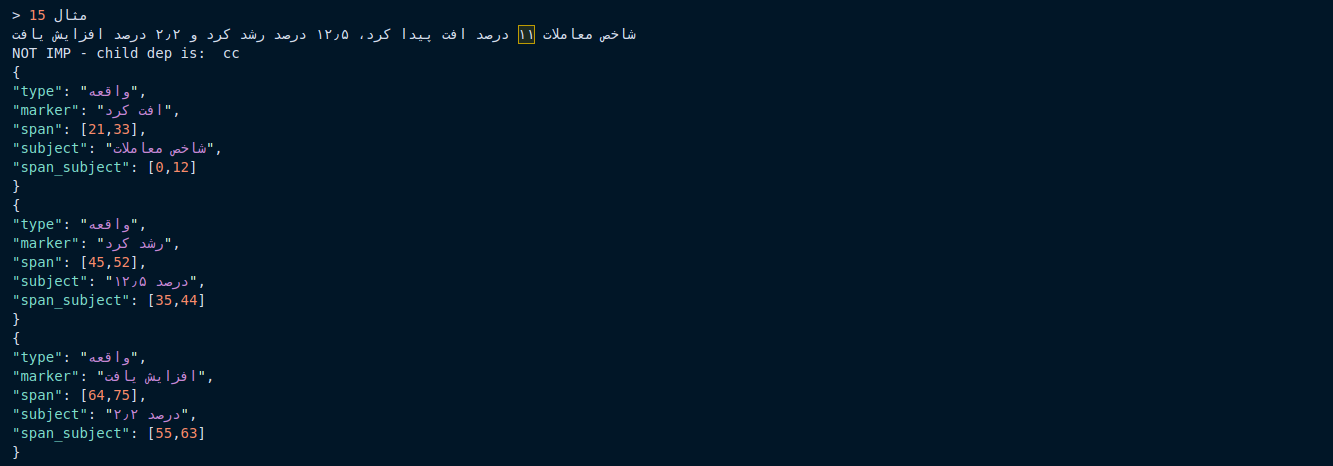
\includegraphics[scale=0.5, trim ={0 0 17cm 0}, clip]{images/15.png}
\end{center}







\subsection*{به دست آوردن کلمات کلیدی}

در این قسمت، به دنبال کلمات کلیدی از پیش تعیین شده‌ای در متن می‌گردیم. این کلمات در 
دسته‌های مختلفی قرار می‌گیرند و اتفاقات مختلفی را گزارش می‌دهند. در صورتی که اتفاقی از 
قلم افتاده باشد، کافی است که یک کلمه‌ی کلیدی مربوط به آن اتفاق را به دسته‌بندی‌های خود 
اضافه کنیم. 

بعضی از کلمه‌های کلیدی دو بخشی‌اند. مانند «عرضه اولیه». در چنین شرایطی، تمام حالات ممکن این 
عبارت کلیدی را نیز پیدا می‌کنیم. برای مثال می‌توانید به خروجی‌های زیر نگاه کنید: 

\begin{center}
	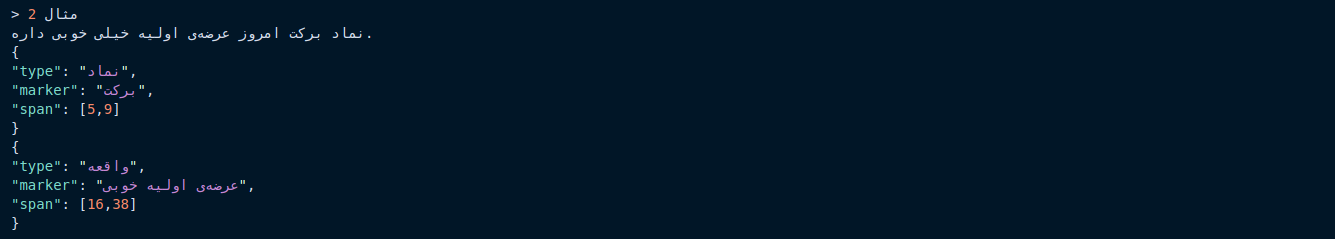
\includegraphics[scale=0.5, trim ={0 0 17cm 0}, clip]{images/IPO1.png}
	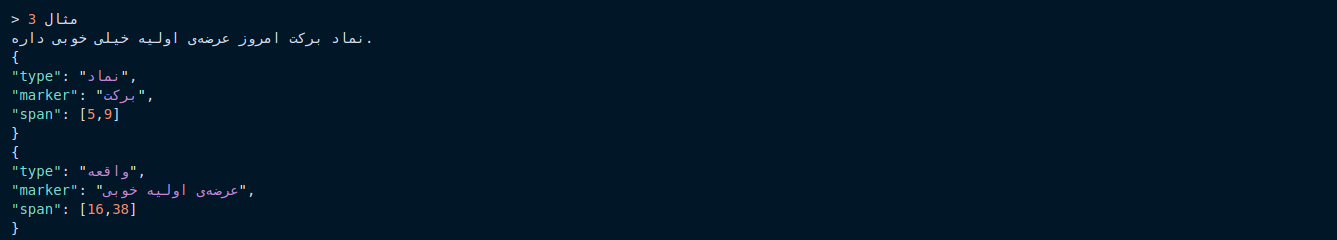
\includegraphics[scale=0.5, trim ={0 0 17cm 0}, clip]{images/IPO2.png}
	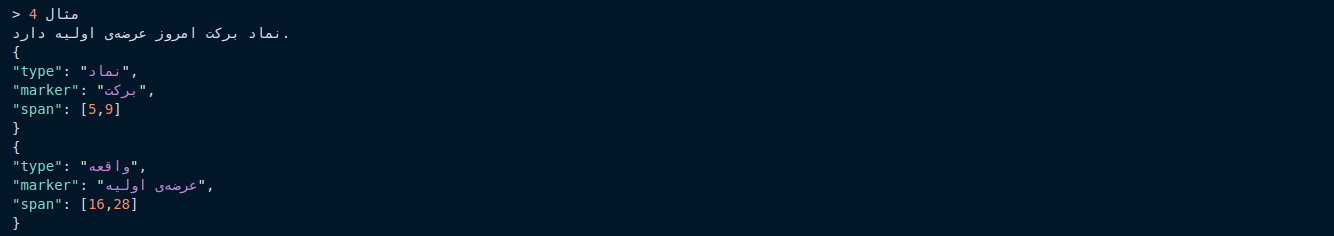
\includegraphics[scale=0.5, trim ={0 0 17cm 0}, clip]{images/IPO3.png}
	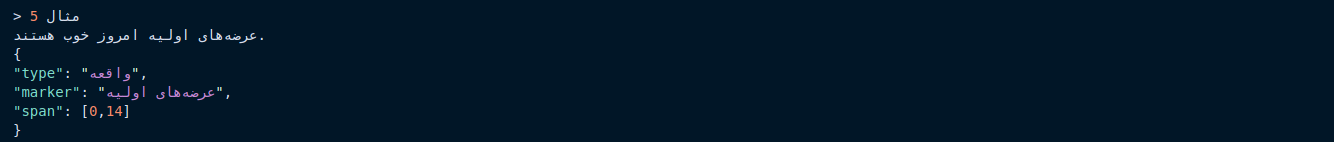
\includegraphics[scale=0.5, trim ={0 0 17cm 0}, clip]{images/IPO4.png}
	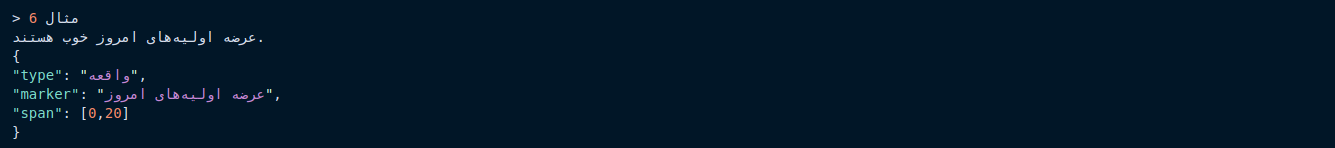
\includegraphics[scale=0.5, trim ={0 0 17cm 0}, clip]{images/IPO5.png}
	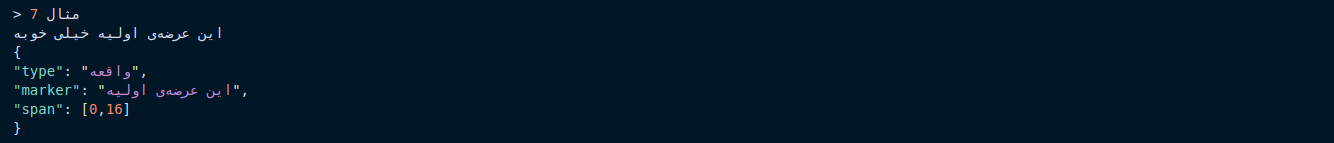
\includegraphics[scale=0.5, trim ={0 0 17cm 0}, clip]{images/IPO6.png}
\end{center}



برای پیدا کردن کلمات کلیدی، از 
regex
ها و کلاس 
Matcher
در کتابخانه‌ی 
spacy
کمک گرفته‌ایم. توکن‌های چند کلمه‌ای پس از این که پیدا شدند، به عنوان یک توکن واحد در نظر 
گرفته می‌شوند تا کنار یک دیگر معنی پیدا کنند. 

برای پیدا کردن نماد‌ها و اسم شرکت‌های بورسی، با 
crawl
کردن توانستیم یک فایل 
csv
تهیه کنیم. سپس به کمک کتابخانه‌ی 
pandas
اسم نماد‌های بورسی و شرکت‌ها را به در متغیر‌های جداگانه ذخیره کردیم، و با 
regex
به دنبال آن‌ها گشتیم. این اسامی در کد ما به عنوان
\lr{Named Entity}
شناخته می‌شوند، و در صورتی استفاده از خروجی
displacy
در کتابخانه
spacy
به صورت زیر نمایش داده می‌شوند: 


\begin{center}
	
\includegraphics[scale=0.5]{images/NE.png}
\end{center}





\subsection*{پیدا کردن متن کامل واقعه}

بعد از این که کلمات کلیدی وقایع را به دست آوردیم،‌ سعی می‌کنیم آن کلمات را گسترش دهیم 
تا شامل یک واقعه‌ی کامل شوند. مثلا، تاثیر یا مثبت به تنهایی یک واقعه تشکیل نمی‌دهند، اما ۵ واحد تاثیر 
مثبت یک واقعه تشکیل می‌دهد. برای این کار، از کتابخانه‌ی
\lr{StanfordNLP}
استفاده می‌کنیم. استنباط ما دو کمک کننده‌ی اساسی دارد. اول
\lr{POS tag}ها
 و دوم استفاده از 
\lr{Dependecy Tree}ها. 
درخت روابط، درختی است که روابط اجزای مختلف یک جمله با هم را نشان می‌دهد. یک مثال از این 
درخت‌ها به صورت زیر است: 

\begin{center}
	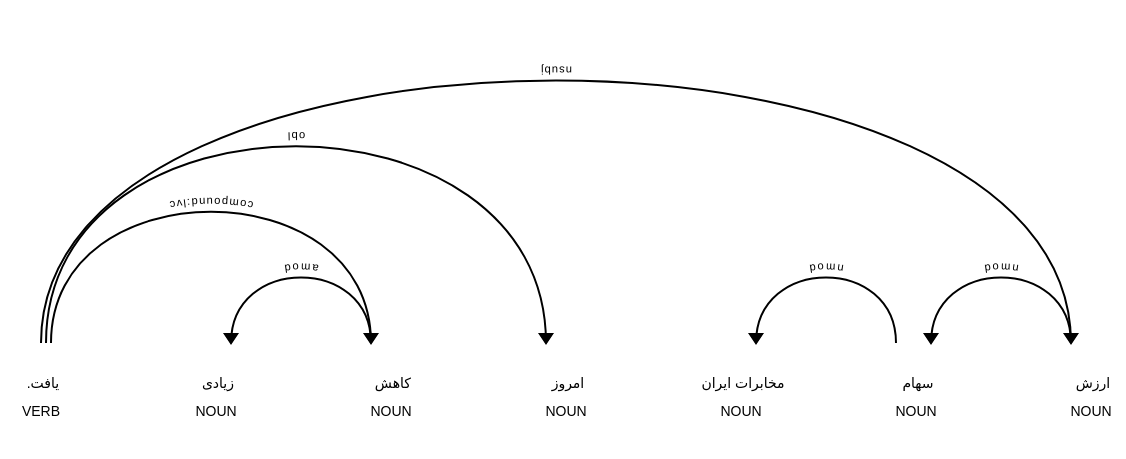
\includegraphics[scale=0.3]{images/DEP.png}
\end{center}


حال وقتی به یک کلمه‌ می‌رسیم، با استفاده از این دو، تشخیص می‌دهیم که واقعه‌ی اصلی چیست. 
برای مثال، وقتی کلمه‌ی کلیدی ما یک مضاف‌الیه است، سعی می‌کنیم هسته‌ی گروه اسمی را به دست 
آوریم و گروه اسمی را خروجی دهیم. مثلا در متن زیر، به جای این که تنها «صف خرید» را 
به عنوان واقعه تشخیص دهیم، کل واقعه یا به عبارتی «ایجاد صف خرید 
در سهم پرشیا» را تشخیص داده‌ایم. 

\begin{center}
	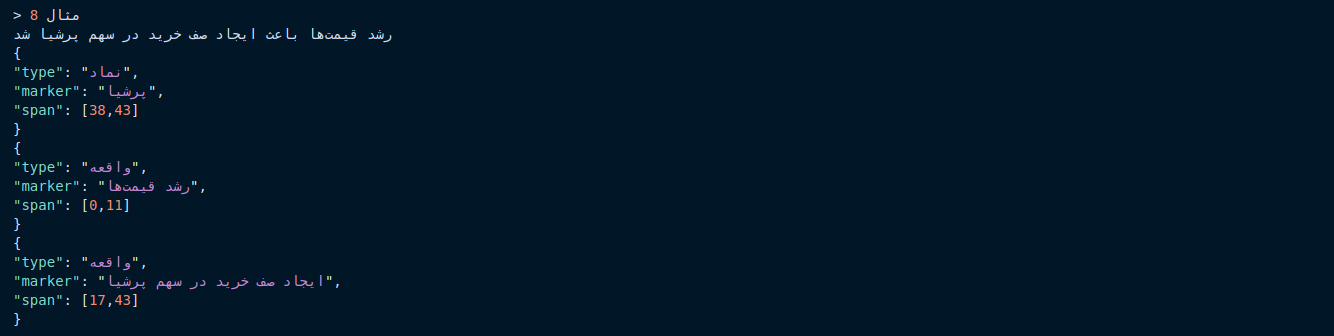
\includegraphics[scale=0.5, trim ={0 0 17cm 0}, clip]{images/8.png}
\end{center}

یا اگر یک فعل مرکب تشخیص دهیم، سعی می‌کنیم فاعل جمله‌ را نیز به دست آوریم تا مفوم 
واقعه کامل باشد. مثلا در ورودی زیر، نه تنها «کاهش زیادی یافتن» را پیدا کرده‌ایم، بلکه 
فاعل آن یعنی «ارزش سهام مخابرات 
ایران» را نیز تشخیص داده‌ایم 
\begin{center}
	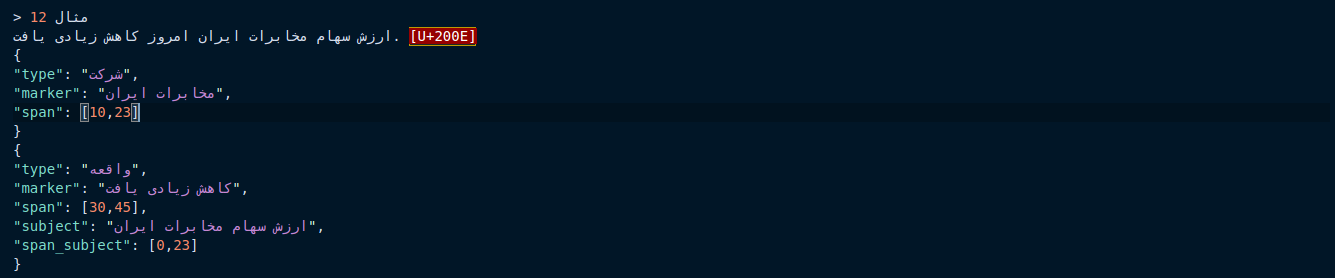
\includegraphics[scale=0.5, trim ={0 0 17cm 0}, clip]{images/12.png}
\end{center}
  توجه کنید که در روند اجرای برنامه هر کجا منطقی برای پیدا کردن اتفاقات کامل‌تر پیاده‌سازی شده متناظرا کد‌های لازم برای حفظ درستی
  \lr{span}
  ها نیز نوشته شده.

\subsection*{خروجی کد و ترکیب وقایع}
\


  در صورتی که دو اتفاق از یک نوع یکسان باشند و هر دو به اتفاقی مشترک اشاره کنند
  این چند اتفاق را با هم ترکیب کرده و در نهایت کامل ‌ترین اتفاق را خروجی می‌دهیم. 
    این کار با الگوریتمی  با زمان اجرای 
 $O(n \log n)$
این کار را انجام می‌دهد. در صورتی که اتفاقات تکراری برای ما مهم نباشد، 
نیازی به اجرای این قسمت از کد نیز نیست و برنامه سریع تر می‌شود. 
نحوه‌ی عملکرد الگوریتم به این صورت است که با بررسی 
  \lr{span}
  اتفاقات رویدادهای مشترک را اجتماع می‌گیرد و از متن اصلی آن‌ها را انتخاب می کند. یک مثال از اجرای این الگوریتم به صورت 
  زیر است که با این که رشد و مثبت هر دو کلمه‌ای کلیدی محسوب می‌شوند، اما 
  ما تنها یک واقعه که «رشد مثبت ...» را تشخیص داده‌ایم. 

\begin{center}
	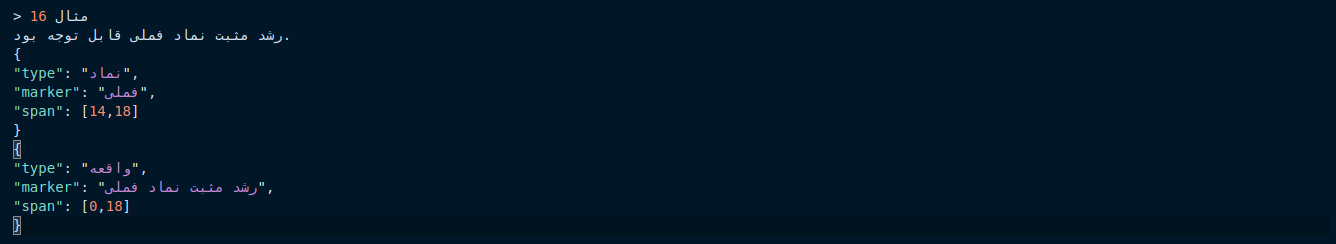
\includegraphics[scale=0.5, trim ={0 0 17cm 0}, clip]{images/16.png}
\end{center}



\subsection*{ملاحضات و بقیه‌ی نکات}
\

کتابخانه‌های مورد نیاز در ابتدای کد نصب می‌شوند، اما در صورتی که بخواهید محیط اجرا را 
عینا شبیه‌سازی کنید می‌توانید از فایل 
requirements 
استفاده کنید. 

\end{document}



